\documentclass[10pt,oneside]{article}

\usepackage{xcolor}
\usepackage{cancel}
\usepackage{bm}
\usepackage{graphicx}
\usepackage[x11names, svgnames]{xcolor} % for colors in handouts, auto loaded in Beamer?
\usepackage{tikz}
\usetikzlibrary{arrows.meta, math, calc, shadows}
\usetikzlibrary{decorations.markings, decorations.fractals, decorations.text} % for chain, etc.
\usetikzlibrary{intersections}
\usepackage{pgfmath}
\usepackage{ifthen}
\usepgfmodule{oo}
\usepgflibrary{shadings}
% \usetikzlibrary{decorations.shapes}
\usepackage[many]{tcolorbox}
\usepackage[absolute,overlay,showboxes]{textpos}
% \usepackage{textpos}
% \textblockorigin{0.0cm}{0.0cm}  %start all at upper left corner
\TPshowboxesfalse

\newcommand\lb{\linebreak}
\newcommand\Ra{\Rightarrow}
\newcommand\cd{\!\cdot\!}
\newcommand\x{\!\times\!}
\newcommand\pars{\par\smallskip}
\newcommand\parm{\par\medskip}
\newcommand\parb{\par\bigskip}
\renewcommand{\deg}{^\circ}

% counter for resuming enumerated list numbers
\newcounter{resumeenumi}
\newcommand{\suspend}{\setcounter{resumeenumi}{\theenumi}}
\newcommand{\resume}{\setcounter{enumi}{\theresumeenumi}}



% https://tex.stackexchange.com/questions/33703/extract-x-y-coordinate-of-an-arbitrary-point-in-tikz
\makeatletter
\providecommand{\gettikzxy}[3]{%
	\tikz@scan@one@point\pgfutil@firstofone#1\relax
	\edef#2{\the\pgf@x}%
	\edef#3{\the\pgf@y}%
}
\makeatother

\makeatletter
\newcommand{\verbatimfont}[1]{\def\verbatim@font{#1}}%
\makeatother

%%%%%%%%%%%%%%%%%%%%%%%%%%%%%%%%%%%%%%%%%%%%%%%%%%%%%%%%%%%%%%%%%%%%%%%%%%%%%%%%


\newcommand{\tb}[4][0.8]{
	\begin{textblock*}{#1}(#2, #3)
		% \raggedright
		#4
	\end{textblock*}
}

\newtcolorbox{statsbox}[2][] { 
  colback=white,
  colbacktitle=structure,
  colframe=structure,
  coltitle=white,  
  top=0.25cm,
	bottom=0.125cm,
	left=0mm,
	right=0mm,
  % fonttitle=\itshape\rmfamily,
  halign=flush left, 
  enhanced,
  drop fuzzy shadow,
  attach boxed title to top left={xshift=3.5mm, yshift=-2mm},
  title={#2}, #1}
\newtcolorbox{redbox}{colback=white, colframe=structure, enhanced, drop fuzzy shadow}
\newtcolorbox{titledbox}[1]{colback=white,colframe=structure,title={#1}}
\newtcbox{\tcb}[1][]{colback=white,boxsep=0pt,top=5pt,bottom=5pt,left=5pt,
		right=5pt, colframe=structure,  enhanced, drop fuzzy shadow, #1}
% tcb title
\newtcbox{\tcbt}[2][]{colback=white,boxsep=0pt,top=5pt,bottom=5pt,left=5pt,
		right=5pt, colframe=structure, enhanced, drop fuzzy shadow,  title={#2}, #1}
% tcb left title
\newtcbox{\tcbtl}[2][]{ colback=white,
  colbacktitle=structure,
  colframe=structure,
  coltitle=white,  
  top=0.25cm,
	bottom=0.125cm,
	left=0mm,
	right=0mm,
  % fonttitle=\bfseries,
  halign=flush left, 
  enhanced,
  drop fuzzy shadow,
  attach boxed title to top left={xshift=3.5mm, yshift=-2mm}, 
	title={#2}, #1}

\newtcbtheorem{myexam}{Example}%
{
	enhanced,
	colback=white,
	colframe=structure,
	% fonttitle=\bfseries,
	fonttitle=\itshape\rmfamily,
	drop fuzzy shadow,
	%description font=\mdseries\itshape,
	attach boxed title to top left={yshift=-2mm, xshift=5mm},
	colbacktitle=structure
	}{exam}% then \pageref{exer:theoexample} references the theo

% \newcommand{\myexample}[2][red]{
% 	% \tcb\tcbset{theostyle/.style={colframe=red,colbacktitle=yellow}}
% 	\begin{myexam}{}{}
% 		#2
% 	\end{myexam}
% 	% \tcbset{colframe=structure,colbacktitle=structure}
% }

\newtcbtheorem{myexer}{Exercise}%
{
	enhanced,
	colback=white,
	colframe=structure,
	% fonttitle=\bfseries,
	drop fuzzy shadow,
	fonttitle=\itshape\rmfamily,
	% description font=\mdseries\itshape,
	attach boxed title to top left={yshift=-2mm, xshift=5mm},
	colbacktitle=structure
	}{exer}



\newcommand{\mini}[2][0.8]{
	\begin{minipage}[c]{#1\columnwidth}
		\raggedright
		#2
	\end{minipage}
}
\newcommand{\minit}[2][0.8]{
	\begin{minipage}[t]{#1\columnwidth}
		% \raggedright
		#2
	\end{minipage}
}

% centered minipage with text \raggedright
%\cmini[width]{content}
\newcommand{\cmini}[2][0.8]{
	\begin{center}
		\begin{minipage}{#1\columnwidth}
			\raggedright
			#2
		\end{minipage}
	\end{center}
}



\newcommand{\fig}[2][1]{% scaled graphic
	\includegraphics[scale=#1]{#2}
}

% centred framed colored box black border
%\cbox[width]{content}
\newcommand{\cbox}[2][1]{% framed centered color box
	\setlength\fboxsep{5mm}
	\setlength\fboxrule{.2 mm}
	\begin{center}
		\fcolorbox{black}{white}{
			\vspace{-0.5cm}
			\begin{minipage}{#1\columnwidth}
				\raggedright
				#2
			\end{minipage}
		}
	\end{center}
	\setlength\fboxsep{0cm}
}

\newcommand{\cfig}[2][1]{% centred, scaled graphic
	\begin{center}
		\includegraphics[scale=#1]{#2}
	\end{center}
}






 \definecolor{saitPurple}{RGB}{112,40,119}
 \definecolor{statsMaroon}{rgb}{0.55, 0, 0}
 \definecolor{saitMaroon}{rgb}{0.55, 0, 0}
 \definecolor{statsRed}{RGB}{224,38,37}
 \definecolor{saitRed}{RGB}{224,38,37}
 \definecolor{saitBlue}{rgb}{0, 0.59, 0.85}
 \definecolor{statsBlue}{rgb}{0, 0.59, 0.85}
 \definecolor{statsDeepBlue}{RGB}{0, 99, 167}
 \definecolor{saitDeepBlue}{RGB}{0, 99, 167}
 \definecolor{saitDeepBlue}{RGB}{0, 99, 167}
 \definecolor{LightGrey}{RGB}{200,200,200}
%  \definecolor{boxBG}{RGB}{236, 227, 227}
%  \definecolor{boxBG}{RGB}{242, 233, 223}
%\Member{startpt}{endpt}{outer fill color}{inner fill color}{stroke}{height}{radius}{linewidth}
\providecommand{\Member}[8]{
  % name the points
  \coordinate(start) at (#1);
  \coordinate(end) at (#2);
  \edef\ofill{#3}%
  \edef\ifill{#4}%
  \edef\stroke{#5}%
  \edef\height{#6} % cm
  \edef\radius{#7} % cm
  \edef\linewidth{#8} % mm

  \coordinate(delta) at ($ (end)-(start) $);
  \gettikzxy{(delta)}{\dx}{\dy}
  \gettikzxy{(start)}{\sx}{\sy}
  \pgfmathparse{veclen(\dx, \dy)} \let\length\pgfmathresult

  \pgfmathparse{\dx==0}%
  % \ifnum low-level TeX for integers
  \ifnum\pgfmathresult=1 % \dx == 0
    \pgfmathsetmacro{\rot}{\dy > 0 ? 90 : -90}
  \else
    \pgfmathsetmacro{\rot}{\dx > 0 ? atan(\dy / \dx) : 180 + atan(\dy / \dx)}
  \fi

  
   
  \shadedraw[transform canvas = { rotate around = {\rot:(\sx,\sy)}}, line width = \linewidth, rounded corners = \radius mm, top color = \ofill, bottom color = \ofill, middle color = \ifill, draw = \stroke] ($ (start)+(-0.5*\height, 0.5*\height) $) -- ++(\height cm +\length pt, 0 ) -- ++(0, -\height) -- ++ (-\height cm -\length pt, 0) -- cycle;


  \shadedraw[ball color = \ofill!50!\ifill, draw = \stroke] (start) circle (\height/8);
  \shadedraw[ball color = \ofill!50!\ifill, draw = \stroke] (end) circle (\height/8);
  %  \pgfresetboundingbox

  
  


}


\newcommand{\PC}[6][0]{%
  \edef\lrotate{#1}%
  \edef\lpin{#2}%
  \edef\lfill{#3}%
  \edef\ldraw{#4}%
  \edef\lscale{#5}%
  \edef\lwidth{#6}% mm
  \edef\h{1}%
  \edef\r{0.3}%
  \begin{scope}[scale=\lscale, rotate=\lrotate]
	\filldraw[draw=\ldraw, fill=\lfill, line width=\lwidth mm] ($ (\lpin) + (0.201*\h+1.0353*\r ,-0.75*\h) $) -- ++(105: 0.77646*\h+0.26795*\r) arc (15:165:\r) -- ++(-105:0.77646*\h+0.26795*\r) -- cycle;

	\shadedraw[ball color=\lfill, draw=\ldraw, line width = \lwidth mm] (\lpin) circle (1.5mm);

	\filldraw[rounded corners=\lscale pt, draw=\ldraw, fill=\lfill, line width=\lwidth mm] ($ (\lpin) - (1,1) $) rectangle +(2,0.25);
  \end{scope}%
}




\usepackage{mathpazo}
\usepackage[letterpaper]{geometry}
\geometry{verbose,tmargin=0.25in,bmargin=0.5in,lmargin=1in,rmargin=1.15in}
\hfuzz 50pt
\setlength{\parindent}{0pt}
\Large

\begin{document}

%%%%%%%%%%%%%%%%%%%%%%%%%%%%%%%%%%%%%%%%%%%%%%%%%%%%%%%%%%%%%%%%%%%%%%%%%%%%%%%%%%%%%%%%%%%%%%%%%%%%
% page 1
%%%%%%%%%%%%%%%%%%%%%%%%%%%%%%%%%%%%%%%%%%%%%%%%%%%%%%%%%%%%%%%%%%%%%%%%%%%%%%%%%%%%%%%%%%%%%%%%%%%%

\begin{textblock*}{6.775in}(1in, 0.225in)
  \cbox{
		\Large\centering
    \textbf{Engineering Statics - 01 Math Review Handout (Instructor Copy)}
  }
\end{textblock*}

\begin{textblock*}{3in}(1in, 1in)
	\large
	\cbox{
		{\bf 1)} Solve $a^2=b^2+c^2$ for $b$.\parm
		\begin{align*}
			b^2 & = a^2-c^2  \\
			b   & = \bm{\pm\sqrt{a^2-c^2}}
		\end{align*}
	}
\end{textblock*}

\begin{textblock*}{3in}(1in, 2.65in)
	\large
	\cbox{
		{\bf 2)} Solve $V=\frac43 \pi r^3$ for $r$. \parm
		\begin{align*}
			r^3 & = \frac{3V}{4\pi}                \\[1em]
			r   & = \bm{\sqrt[3]{\frac{3V}{4\pi}}}
		\end{align*}
	}
\end{textblock*}

\begin{textblock*}{3.75in}(1in, 4.70in)
	\large
	\cbox{
		{\bf 3)} Solve $c^2=a^2+b^2-2bc\cos C$ for $\cos C$.\parm
		\begin{align*}
			2bc\cos C & = a^2+b^2-c^2                  \\[1em]
			\bm{\cos C}    & \bm{=\frac{a^2+b^2-c^2}{2bc}}
		\end{align*}
	}
\end{textblock*}





\begin{textblock*}{3.75in}(1in, 6.625in)
	\large
	\cbox{
		{\bf 4)} Solve $b^2=a^2+c^2-2ac\cos B$ for $B$.\parm
		\begin{align*}
			2ac\cos B & = a^2+c^2-b^2                                   \\[1em]
			\cos B    & = \frac{a^2+c^2-b^2}{2bc}                       \\[1em]
				\bm B         & \bm{ = \cos^{-1}\left(\frac{a^2+c^2-b^2}{2bc}\right)}
		\end{align*}
	}
\end{textblock*}




%%%%%%%%%%%%%%%%%%%%%%%%%%%%%%%%%%%%%%%%%%%%%%%%%%%%%%%%%%%%%%%%%%%%%%%%%%%%%%%%%%%%%%%%%%%%%%%%%%%%
% page 2
%%%%%%%%%%%%%%%%%%%%%%%%%%%%%%%%%%%%%%%%%%%%%%%%%%%%%%%%%%%%%%%%%%%%%%%%%%%%%%%%%%%%%%%%%%%%%%%%%%%%
.\newpage

\begin{textblock*}{6.5in}(1in, 0.225in)
	\large
	\cbox{
		{\bf 5)}  Solve the equation for $h_L$, then evaluate $h_L$ using the values $Q=135$, $C=120$, $D=202.7$ and $L=1200$\parm
		\begin{align*}
			Q                                             & = \frac{CD^{2.63}\left(\frac{h_L}{L}\right)^{0.54}}{279000} \\[1em]
			\Rightarrow \left(\frac{h_L}{L}\right)^{0.54} & = \frac{279000Q}{CD^{2.63}}                                 \\[1em]
			\Rightarrow \frac{h_L}{L}                     & = \left(\frac{279000Q}{CD^{2.63}}\right)^{1/0.54}           \\[1em]
			\Rightarrow \bm{ h_L}                               & \bm{= L\left(\frac{279000Q}{CD^{2.63}}\right)^{1.85}}         \\\\
			h_L &= 1200\left(\frac{279000\times 135}{120\times 202.7^{2.63}}\right)^{1.85} \\[1em]
			&=105.73 \\[1em]
			\bm{h_L} &\bm{= 106}
		\end{align*}
	}
\end{textblock*}


\begin{textblock*}{3.25in}(1in, 5.5in)
	\large
	\cbox{
		{\bf 6)} Use the Pythagorean Theorem to determine the lengths of $CE$ and $CB$\parm
		\large
		\begin{align*}
			CE^2 & = EF^2+CF^2                              \\
			     & = (3.00\,\mathsf{m})^2+3.75^2                          \\
			CE   & = 4.8023                                 \\
			     & = \bm{4.80\,\mathsf{ m}} \\\\
			CB^2 & = 1.25^2+3.00^2                          \\
			CB   & = 3.2500                                 \\
			     & = \bm{3.25\,\mathsf{ m}}
		\end{align*}
	}


\end{textblock*}

\begin{textblock*}{2.625in}(4.875in, 5.5in)  
	\cbox{
		\centering
    \vspace{-0.25cm}
    
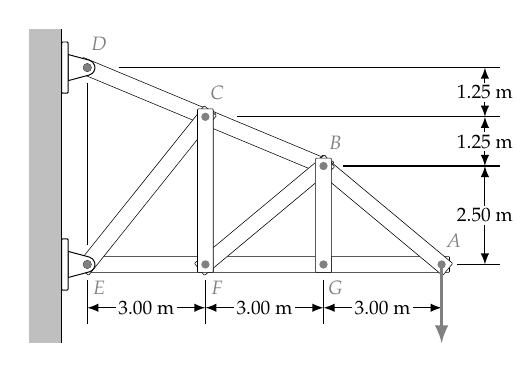
\begin{tikzpicture}



	\def\offset{0.2}
	
	\coordinate (E) at (0,0);
	\coordinate (F) at (1.5,0);
	\coordinate (G) at (3,0);
	\coordinate (A) at (4.5,0);
	\coordinate (B) at (3,1.25);
	\coordinate (C) at (1.5,1.875);
	\coordinate (D) at (0,2.5);
	\coordinate (Right) at ($ (A)+(0.75,0)$);
	\coordinate (Bottom) at ($ (A)+(0,-0.75)$);

	\filldraw[gray!50] ($(D)+(-0.325,0.5)$) rectangle ($(E)+(-.75,-1)$);
	\draw ($(D)+(-0.325,0.5)$) -- ($(E)+(-0.325,-1)$);


	\gettikzxy{(A)}{\ax}{\ay}
	\gettikzxy{(B)}{\bx}{\by}
	\gettikzxy{(C)}{\cx}{\cy}
	\gettikzxy{(D)}{\ddx}{\ddy}
	\gettikzxy{(E)}{\ex}{\ey}
	\gettikzxy{(F)}{\fx}{\fy}
	\gettikzxy{(G)}{\gx}{\gy}
	\gettikzxy{(Right)}{\rx}{\ry}
	\gettikzxy{(Bottom)}{\bbx}{\bby}

	\draw ($ (A)+(\offset,0)$) -- (\rx,\ay);
	\draw ($ (B)+(1.25*\offset,0)$) -- (\rx,\by);
	\draw ($ (C)+(2*\offset,0)$) -- (\rx,\cy);
	\draw ($ (D)+(2*\offset,0)$) -- (\rx,\ddy);
	\draw ($ (D)+(0, -\offset)$) -- (\ex,\ey+1.25*\offset cm);
	\draw ($ (E)+(0, -\offset)$) -- (\ex,\bby);
	\draw ($ (F)+(0, -\offset)$) -- (\fx,\bby);
	\draw ($ (G)+(0, -\offset)$) -- (\gx,\bby);
	\draw ($ (A)+(0, -\offset)$) -- (\ax,\bby);

	\small
	\draw[latex-latex] (\ex,\bby+\offset cm) -- node[fill=white, inner sep=0.35mm] {\scriptsize $3.00$ m}(\fx,\bby+\offset cm);
	\draw[latex-latex] (\fx,\bby+\offset cm) -- node[fill=white, inner sep=0.35mm] {\scriptsize $3.00$ m}(\gx,\bby+\offset cm);
	\draw[latex-latex] (\gx,\bby+\offset cm) -- node[fill=white, inner sep=0.35mm] {\scriptsize $3.00$ m}(\ax,\bby+\offset cm);
	\draw[latex-latex] (\rx-\offset cm,\ay) -- node[fill=white, inner sep=0.35mm] {\scriptsize $2.50$ m}(\rx-\offset cm,\by);
	\draw[latex-latex] (\rx-\offset cm,\by) -- node[fill=white, inner sep=0.35mm] {\scriptsize $1.25$ m}(\rx-\offset cm,\cy);
	\draw[latex-latex] (\rx-\offset cm,\cy) -- node[fill=white, inner sep=0.35mm] {\scriptsize $1.25$ m}(\rx-\offset cm,\ddy);
	\normalsize

	 
	 \Member{B}{C}{white}{white}{black}{0.2}{0.095}{0.2}
	 \Member{C}{D}{white}{white}{black}{0.2}{0.095}{0.2}
	 \Member{A}{G}{white}{white}{black}{0.2}{0.095}{0.2}
	 \Member{A}{B}{white}{white}{black}{0.2}{0.095}{0.2}
	 \Member{F}{G}{white}{white}{black}{0.2}{0.095}{0.2}
	 \Member{F}{E}{white}{white}{black}{0.2}{0.095}{0.2}
	 \Member{B}{F}{white}{white}{black}{0.2}{0.095}{0.2}
	 \Member{B}{G}{white}{white}{black}{0.2}{0.095}{0.2}
	 \Member{C}{E}{white}{white}{black}{0.2}{0.095}{0.2}
	 \Member{C}{F}{white}{white}{black}{0.2}{0.095}{0.2}

	\PC[-90]{D}{white}{black}{0.325}{0.125}
	\PC[-90]{E}{white}{black}{0.325}{0.125}

	\draw[very thick, gray, -latex] (A) -- +(0,-1);

	\fill[gray] (A) circle (1.5pt) node[xshift=1.5mm, yshift=3mm] {\scriptsize $A$};
	\fill[gray] (B) circle (1.5pt) node[xshift=1.5mm, yshift=3mm] {\scriptsize $B$};
	\fill[gray] (C) circle (1.5pt) node[xshift=1.5mm, yshift=3mm] {\scriptsize $C$};
	\fill[gray] (D) circle (1.5pt) node[xshift=1.5mm, yshift=3mm] {\scriptsize $D$};
	\fill[gray] (E) circle (1.5pt) node[xshift=1.5mm, yshift=-3mm] {\scriptsize $E$};
	\fill[gray] (F) circle (1.5pt) node[xshift=1.5mm, yshift=-3mm] {\scriptsize $F$};
	\fill[gray] (G) circle (1.5pt) node[xshift=1.5mm, yshift=-3mm] {\scriptsize $G$};
\pgfresetboundingbox
\draw[white] ($ (D)+ (-0.75,0.5) $) rectangle ($ (A)+(0.75,-1) $);

\end{tikzpicture}

    \vspace{-0.125cm}
	}
\end{textblock*}


%%%%%%%%%%%%%%%%%%%%%%%%%%%%%%%%%%%%%%%%%%%%%%%%%%%%%%%%%%%%%%%%%%%%%%%%%%%%%%%%%%%%%%%%%%%%%%%%%%%%
% page 3
%%%%%%%%%%%%%%%%%%%%%%%%%%%%%%%%%%%%%%%%%%%%%%%%%%%%%%%%%%%%%%%%%%%%%%%%%%%%%%%%%%%%%%%%%%%%%%%%%%%%
.\newpage

\begin{textblock*}{6.75in}(1in, 0.225in)
	\large
	\cbox{
		{\bf 7)} Use the tangent function to calculate $\angle CEF$\parm		
		$$ \angle CEF = \tan^{-1}\left(\frac{CF}{EF}\right) =  \tan^{-1}\left(\frac{3.75\,\mathsf{m}}{3.00\,\mathsf{m}}\right) = 51.340\deg = \bm{51.3\deg}  $$
	}
\end{textblock*}

\begin{textblock*}{6.75in}(1in, 1.75in)
	\large
	\cbox{
		{\bf 8)} Use $\angle CEF$ just found and the sine function to verify the length of $CE$ found above.\parm
		\begin{align*}
			\frac{CD}{\sin 90\deg} & = \frac{CF}{\sin \angle CEF}                 \\[1em]
			\Rightarrow CE           & = \frac{(3.75\,\mathsf{m})\sin 90\deg}{\sin 51.340\deg} 		\\[1em]
			                         & = 4.8024                                     \\[1em]
			            \bm{CE}     & = \bm{4.80\,\mathsf{m}}
		\end{align*}
	}
\end{textblock*}


\begin{textblock*}{6.75in}(1in, 4.75in)
	\large
	\cbox{
		{\bf 9)} Use the cosine function and the length of $BC$ found earlier to calculate the angle, $\theta$, between $BC$ and the horizontal.\parm		
		\begin{align*}
			(1.25\,\mathsf{m})^2 &= (3.00\,\mathsf{m})^2 + (3.25\,\mathsf{m})^2-2(3.00\,\mathsf{m})(3.25\,\mathsf{m})\cos\theta \\[0.5em]
			\Rightarrow \cos\theta &= \frac{(3.00\,\mathsf{m})^2 + (3.25\,\mathsf{m})^2-(1.25\,\mathsf{m})^2}{2(3.00\,\mathsf{m})(3.25\,\mathsf{m})} \\[0.5em]
			&= 0.92308\\\\
			\Rightarrow \theta &= 22.619\deg\\[0.5em]			
			\bm{\theta} & \bm{=22.6\deg}
		\end{align*}
	}
\end{textblock*}


\begin{textblock*}{6.75in}(1in, 8.125in)
	\large
	\cbox{
		{\bf 10)} Use the tangent function to verify the previous result.\parm
		
		$$ \theta = \tan^{-1}\left(\frac{1.25\,\mathsf{m}}{3.00\,\mathsf{m}}\right)= 22.620 =\bm{22.6\deg} $$
	}
\end{textblock*}

%%%%%%%%%%%%%%%%%%%%%%%%%%%%%%%%%%%%%%%%%%%%%%%%%%%%%%%%%%%%%%%%%%%%%%%%%%%%%%%%%%%%%%%%%%%%%%%%%%%%
% page 4
%%%%%%%%%%%%%%%%%%%%%%%%%%%%%%%%%%%%%%%%%%%%%%%%%%%%%%%%%%%%%%%%%%%%%%%%%%%%%%%%%%%%%%%%%%%%%%%%%%%%
.\newpage

\begin{textblock*}{4in}(1in, 0.225in)
	\large
	\cbox{
		{\bf 11)} Using the sine rule, find $\angle ACB$.\parm
		\large
		\begin{align*}
			\frac{\angle ACB}{3.35\,\mathsf{cm}} & = \frac{\sin 54.7\deg}{5.26\,\mathsf{cm}}                           \\
			\Rightarrow\angle ACB   & = \sin^{-1}\left(\frac{(3.35\,\mathsf{cm})\sin 54.7\deg}{5.26\,\mathsf{cm}}\right) \\
			                        & = 31.318\deg                                           \\
			                        & = \bm{31.3\deg}
		\end{align*}
	}
\end{textblock*}

\begin{textblock*}{2in}(5.675in, 0.225in)
	\cbox{
		\centering
		% !TEX root = ../../Beamer/statikz/statikz.tex


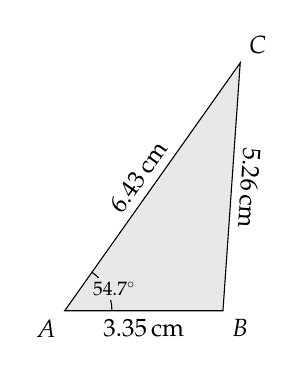
\begin{tikzpicture}[scale=0.6]

	\coordinate (A) at (0,0);
	\coordinate (B) at ($ (A)+(3.35, 0)$);
	\coordinate (C) at ($ (A)+(54.7:6.43)$);
	
  

	\small
	\filldraw[fill=Gainsboro!65, draw=black] (A) -- (B) --  (C) --  cycle;
  
	\path (A) -- (C) node[midway, sloped, above] {$6.43\,$cm};
	\path (C) -- (B) node[midway, sloped, above, rotate=180] {$5.26\,$cm};
	\path (A) -- (B) node[midway, sloped, below] {$3.35\,$cm};
	\draw[below right] (B) node {$B$};
	\draw[below left] (A) node {$A$};
	\draw[above right] (C) node {$C$};

	\draw ($ (A)+(54.7:1) $) arc (54.7:0:1)node[midway, fill=Gainsboro!65, inner sep=0.5mm,xshift=1mm] {\scriptsize $ 54.7\deg $};
  

	% \node[xshift=-0.5cm, yshift=0.15cm] at (C) {$\theta $};



\end{tikzpicture}

	}
\end{textblock*}

\begin{textblock*}{6.75in}(1in, 2.75in)
	\large
	\cbox{
		{\bf 12)} Using the sine rule, find $\angle ABC$.\parm
		\begin{align*}
			\frac{\angle ABC}{6.43\,\mathsf{cm}} & = \frac{\sin 54.7\deg}{5.26\,\mathsf{cm}}                           \\[1em]
			\Rightarrow\angle ABC   & = \sin^{-1}\left(\frac{(6.43\,\mathsf{cm})\sin 54.7\deg}{5.26\,\mathsf{cm}}\right) \\
			                        & = 86.091\deg \\[1em]
							\bm{\angle ABC} &  \bm{=86.1\deg}\qquad\text{(or $93.9(09)\deg$\ldots)}
		\end{align*}
	}
\end{textblock*}

\begin{textblock*}{6.75in}(1in, 5.625in)
	\large
	\cbox{
		{\bf 13)} Sum the interior angles of the triangle.\parm		 
		$$ = 54.7\deg+ 33.318\deg + 86.091\deg = \bm{172.11\deg} $$
		\parm
		(Explain it's due to choice of $\angle ABC=86.1\deg$ from the inverse $\sin$ above. Or wait until $\angle ABC$ is found from the $\cos$ rule in the next exercise.)
	}
\end{textblock*}

\begin{textblock*}{6.75in}(1in, 7.625in)
	\large
	\cbox{
		{\bf 14)} Using the cosine rule, determine $\angle ABC$ \pars
		{\bf 15)} Compare with the earlier value calculated for $\angle ABC$ 
		% 10) Compare the value for $\angle ABC$ with the value calculated earlier.\parm\Large
		\begin{align*}
			(6.43\,\mathsf{cm})^2 & = (3.35\,\mathsf{cm})^2+(5.26\,\mathsf{cm})^2-2(3.35\,\mathsf{cm})(5.26\,\mathsf{cm})\cos\angle ABC \\[0.35em]
			\Rightarrow \angle ABC & = \cos^{-1}\left[\frac{(3.35\,\mathsf{cm}^2)+(5.26\,\mathsf{cm})^2-(6.43\,\mathsf{cm})^2}{2(3.35\,\mathsf{cm})(5.26\,\mathsf{cm})}\right]       \\[0.35em]
			    & =93.994\deg \\[0.35em]
			\bm{\angle ABC}    & \bm{=94.0\deg}
		\end{align*}
		\vspace{-0.25em}
		(Slightly different since from $93.9\deg$ since $54.7\deg$ is accurate to $3$ significant digits and not a more precise given value.)
	}
\end{textblock*}

%%%%%%%%%%%%%%%%%%%%%%%%%%%%%%%%%%%%%%%%%%%%%%%%%%%%%%%%%%%%%%%%%%%%%%%%%%%%%%%%%%%%%%%%%%%%%%%%%%%%
% page 5
%%%%%%%%%%%%%%%%%%%%%%%%%%%%%%%%%%%%%%%%%%%%%%%%%%%%%%%%%%%%%%%%%%%%%%%%%%%%%%%%%%%%%%%%%%%%%%%%%%%%
.\newpage




\begin{textblock*}{2.725in}(5.075in, 0.225in)
	\cbox{
    \vspace{-0.25cm}
		\centering
		


\scalebox{0.75}{
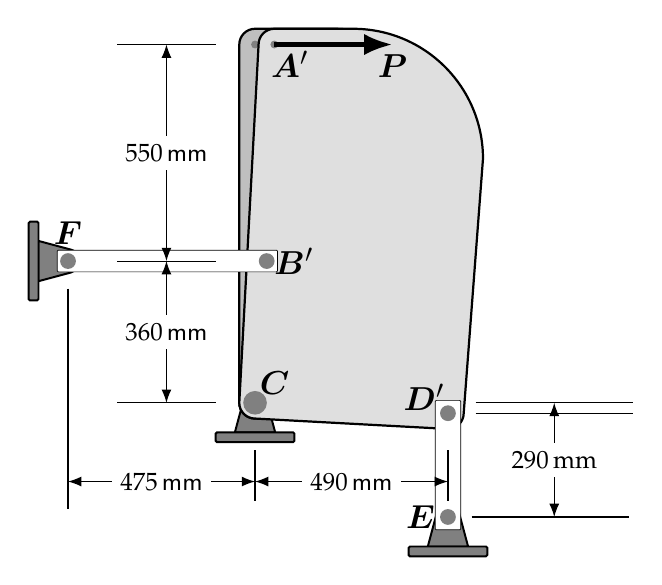
\begin{tikzpicture}[scale=1]

	\coordinate (C) at (0,0);
	\coordinate (B) at ($ (C)+(90:1.8)  $);
	\coordinate (BB) at ($ (B)+(0:0.148)  $);
	\coordinate (A) at ($ (B)+(90:2.75) $);
	\coordinate (AA) at ($ (A)+(0:0.245) $);
  \coordinate (D) at ($ (C)+(0:2.45) $);
  \coordinate (DD) at ($ (D)+(-90:.132) $);
	\coordinate (E) at ($ (D)+(-90:1.45) $);
	\coordinate (F) at ($ (B)+(180:2.375) $);
	\def\d{0.2cm}

	\gettikzxy{(A)}{\ax}{\ay}
	\gettikzxy{(AA)}{\aax}{\aay}
  \gettikzxy{(B)}{\bx}{\by}
  \gettikzxy{(BB)}{\bbx}{\bby}
  \gettikzxy{(C)}{\cx}{\cy}
  \gettikzxy{(D)}{\ddx}{\ddy}
  \gettikzxy{(DD)}{\dddx}{\dddy}
  \gettikzxy{(E)}{\ex}{\ey}
  \gettikzxy{(F)}{\fx}{\fy}

	\PC[270]{F}{gray}{black}{0.5}{0.25}
	\PC{E}{gray}{black}{0.5}{0.25}
	\PC{C}{gray}{black}{0.5}{0.25}

	\small


		\filldraw[thick, fill=gray!50, draw=black] (\cx-\d, \cy)--(\cx-\d, \ay)arc(180:90:\d)--+(1,0)arc(90:0:1.65)--(\ddx+\d, \ddy)arc(0:-90:\d)--(\cx, \cy-\d)arc(270:180:\d);


		
		\draw[thin] (\ddx+0.35cm, \ddy) -- +(2,0);
		\draw[Latex-Latex] (\ddx+1.35cm,\ddy) -- node[fill=white] { $290\,\text{mm}$}(\ddx+1.35cm,\ey);
	
		\fill [gray] (B) circle (0.1cm) node[black, xshift=0.3cm] {\large $\bm B$};	
		\fill [gray] (A) circle (0.05cm) node[black, xshift=0.2cm, yshift=-0.25cm] {\large $\bm A$};
		\fill [gray] (D) circle (0.1cm) node[black, xshift=-0.3cm, yshift=0.2cm] {\large $\bm D$};



		\filldraw[thick, gray!25, draw=black] (\cx-\d, \cy)--(\aax-\d, \aay)arc(180:90:\d)--+(1,0)arc(90:0:1.65)--(\dddx+\d, \dddy)arc(0:-90:\d)--(\cx, \cy-\d)arc(270:180:\d);
		% \draw[Latex-Latex] (\dddx+1.35cm,\dddy) -- node[fill=white] { $290\,\mathsf{mm}-\delta_{DE}$}(\ddx+1.35cm,\ey);
		\draw[thin] (\dddx+0.35cm, \dddy) -- +(2,0);

		\Member{F}{BB}{white}{white}{black}{0.275}{.125}{0.25}
		\Member{DD}{E}{white}{white}{black}{0.325}{.125}{0.25}
		
		\fill [gray] (BB) circle (0.1cm) node[black, xshift=0.35cm] {\large $\bm B'$};
		\fill [gray] (AA) circle (0.05cm) node[black, xshift=0.2cm, yshift=-0.25cm] {\large $\bm A'$};
		\fill [gray] (DD) circle (0.1cm) node[black, xshift=-0.3cm, yshift=0.2cm] {\large $\bm D'$};
		\draw[-Latex, ultra thick, black] (AA)--+(1.5,0)node[black, below]{\large $\bm P$};



	\draw[Latex-Latex] (\cx-1.125cm,\ddy) -- node[fill=white] { $360\,\mathsf{mm}$}(\cx-1.125cm,\by);
	\draw[Latex-Latex] (\cx-1.125cm,\ay) -- node[fill=white] { $550\,\mathsf{mm}$}(\cx-1.125cm,\by);
	\draw[Latex-Latex] (\fx,\cy-1cm) -- node[fill=white] { $475\,\mathsf{mm}$}(\cx,\cy-1cm);
	\draw[Latex-Latex] (\cx,\cy-1cm) -- node[fill=white] { $490\,\mathsf{mm}$}(\ddx,\cy-1cm);

	\draw[thin] (\ax-0.5cm, \ay) -- +(-1.25, 0);
	\draw[thin] (\bx-0.5cm, \by) -- +(-1.25, 0);
	\draw[thin] (\cx-0.5cm, \cy) -- +(-1.25, 0);
	\draw[thin] (\cx, \cy-0.6cm) -- +(0, -0.65);
	\draw[thin] (\ddx, \ddy-0.6cm) -- +(0, -0.65);
	\draw[thin] (\ex+0.3cm, \ey) -- +(2,0);
	\draw[thin] (\fx, \fy-0.35cm) -- (\fx, \cy-1.35cm);
	
	\large 
	\fill [gray] (E) circle (0.1cm) node[black, xshift=-0.35cm] {$\bm E$};
	\fill [gray] (F) circle (0.1cm) node[black, yshift=0.35cm] {$\bm F$};
	\fill [gray] (C) circle (0.15cm) node[black, xshift=0.25cm, yshift=0.25cm] {\large $\bm C$};
	



\end{tikzpicture}
}
    \vspace{-0.25cm}
	}
\end{textblock*}

\begin{textblock*}{3.5125in}(1in, 0.225in)
	\large
	\cbox{
		When horizontal force $P$ is applied at $A$, $ABCD$ rotates about $C$ and $A$ deflects 2.45~mm horizontally rightwards. \parm
		Assume that $BF$ remains horizontal and that $DE$ remains vertical.\parm
		{\bf 16)} Determine $\delta_{BF}$, the change in length of $BF$. \parm
		$\triangle CAA'$, $\triangle CBB'$ and $\triangle CDD'$ are all similar.
		\begin{align*}
			\frac{\delta_{BF}}{2.45\,\mathsf{mm}}    & = \frac{360\,\mathsf{mm}}{360\,\mathsf{mm}+550\,\mathsf{mm}}            \\[0.5em]
			\Rightarrow \delta_{BF} & =0.96923\,\mathsf{mm}                        \\[0.5em]
			      \bm{\delta_{BF}} 	&\bm{=0.969}\text{ \bfseries mm}			
		\end{align*}
	}
\end{textblock*}

\begin{textblock*}{3.5125in}(1in, 3.45in)
	\large
	\cbox{		
		{\bf 17)} Determine $\delta_{DE}$, the change in length of $DE$.\pars
		\begin{align*}
			\frac{\delta_{DE}}{2.45\,\mathsf{mm}}    & = \frac{490\,\mathsf{mm}}{360\,\mathsf{mm}+550\,\mathsf{mm}}            \\[0.5em]
			\Rightarrow \delta_{BF} & =1.3192                          \\[0.5em]
			                            & = \bm{1.32}\text{ \bfseries mm}
		\end{align*}
	}
\end{textblock*}
	

\begin{textblock*}{1.77in}(5.95in, 5.675in)
	\cbox{
    \vspace{-0.25cm}
		\centering
		% !TEX root = ../../Beamer/statikz/statikz.tex


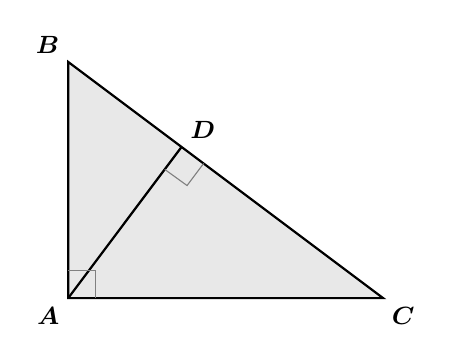
\begin{tikzpicture}[scale=1]

	\coordinate (A) at (0,0);
	\coordinate (B) at (0,3);
	\coordinate (C) at (4,0);
	% super cool tikzlibrary{calc} to get the point D on BC perpendicular from A
	\coordinate (D) at ($ (B)!(A)!(C) $);

	
  

	\small
	\filldraw[thick, fill=Gainsboro!65, draw=black] (A) -- (B) --  (C) --  cycle;
	\filldraw[thick, fill=Gainsboro!65, draw=black] (A) -- (D);
	\draw[gray, thin] ($ (D)+(-36.87:0.35) $) -- ++(233.13:0.35)-- +(144.13:0.35);
	\draw[gray, thin] (0,0.35) -- (0.35,0.35)-- (0.35,0);
  
	% \path (A) -- (C) node[midway, sloped, above] {$6.43\,$cm};
	% \path (C) -- (B) node[midway, sloped, above, rotate=180] {$5.26\,$cm};
	% \path (A) -- (B) node[midway, sloped, below] {$3.35\,$cm};
	\draw[below left] (A) node {$\bm A$};
	\draw[above left] (B) node {$\bm B$};
	\draw[below right] (C) node {$\bm C$};
	\draw[above right] (D) node {$\bm D$};

	% \draw ($ (A)+(54.7:1) $) arc (54.7:0:1)node[midway, fill=Gainsboro!65, inner sep=0.5mm,xshift=1mm] {\scriptsize $ 54.7\deg $};
  

	% \node[xshift=-0.5cm, yshift=0.15cm] at (C) {$\theta $};



\end{tikzpicture}

    \vspace{-0.5cm}
	}
\end{textblock*}

\begin{textblock*}{4.35in}(1in, 5.675in)
	\large
	\cbox{
    {\bf 18)} Show that right triangles $\triangle ABC$, $\triangle ABD$ and $\triangle ACD$ all have the same angles (i.e. they are all similar).
    \begin{align*}
			\text{Let }\angle DCA  & = \theta          \\[0.35em]
			\text{Then }\angle DAC & = 90^\circ-\theta \\[0.35em]
			\Rightarrow \angle DAB & = \theta          \\[0.35em]
			\Rightarrow \angle DBA & = 90^\circ-\theta
		\end{align*}
		Each of the three triangles has angles $\theta$, $90^\circ-\theta$ and $90^\circ$, so they are similar.
	}
\end{textblock*}

\begin{textblock*}{6.775in}(1in, 8.5in)
	\large
	\cbox{
    \vspace{-0.25cm}
		{\bf 19)} Given that $AC=100\text{ mm}$ and $AD=65\text{ mm}$, determine $\angle ACD$ and $\angle ABD$.
		\begin{align*}
			\angle ACD & = \sin^{-1}\left(\frac{65\,\mathsf{mm}}{100\,\mathsf{mm}}\right) = 40.542\deg = \bm{40.5\deg}. \\
			\angle ABD & = 90\deg- 40.542\deg = 49.458\deg = \bm{49.5\deg}.           
		\end{align*}
	}
\end{textblock*}

%%%%%%%%%%%%%%%%%%%%%%%%%%%%%%%%%%%%%%%%%%%%%%%%%%%%%%%%%%%%%%%%%%%%%%%%%%%%%%%%%%%%%%%%%%%%%%%%%%%%
% page 6
%%%%%%%%%%%%%%%%%%%%%%%%%%%%%%%%%%%%%%%%%%%%%%%%%%%%%%%%%%%%%%%%%%%%%%%%%%%%%%%%%%%%%%%%%%%%%%%%%%%%
.\newpage

\begin{textblock*}{6.75in}(1in, 0.225in)
	\large
	\cbox{
   {\bf 20)} Find the remaining lengths: $AB$, $BD$ and $CD$.
	 \begin{gather*}
			\frac{AB}{100\,\mathsf{mm}} = \tan 40.542\deg \Rightarrow AB = 85.263\,\mathsf{mm}= \bm{85.2\,\mathsf{mm}}\\[0.75em]
			\frac{BD}{65\,\mathsf{mm}} = \tan 40.542\deg \Rightarrow BD = 55.598\,\mathsf{mm} = \bm{55.6\,\mathsf{mm}}\\[0.75em]
			\frac{DC}{65\,\mathsf{mm}} = \tan \left(90\deg-40.542\deg\right) \Rightarrow DC = 75.993\,\mathsf{mm} = \bm{76.0\,\mathsf{ mm}}
		\end{gather*}
	}
\end{textblock*}

\begin{textblock*}{6.75in}(1in, 2.4in)
	\large
	\cbox{    
		{\bf 21)} Verify the lengths found above by using the Pythagorean Theorem on $\triangle ABC$
		\begin{align*}
			AC^2 + AB^2 &= (100\,\mathsf{mm})^2 + (85.263\,\mathsf{mm})^2 
			= 17270\,\mathsf{mm^2} 
			= BC^2 \\[0.25em]
			\Rightarrow BC &= 131.42\,\mathsf{mm} \\
			BD+CD &= 55.598\,\mathsf{mm}+75.993\,\mathsf{mm} 
			= BC 
			\Rightarrow BC = 131.59\,\mathsf{mm}
		\end{align*}
			An accumulation of rounding errors can start to cause differences when there are so many calculations and so many rounded intermediate values to use.   
	}

\end{textblock*}

\begin{textblock*}{2.26in}(5.5in, 4.45in)
	\cbox{
		\centering
		\resizebox{2.4in}{!}{
		% !TEX root = ../../Beamer/statikz/statikz.tex


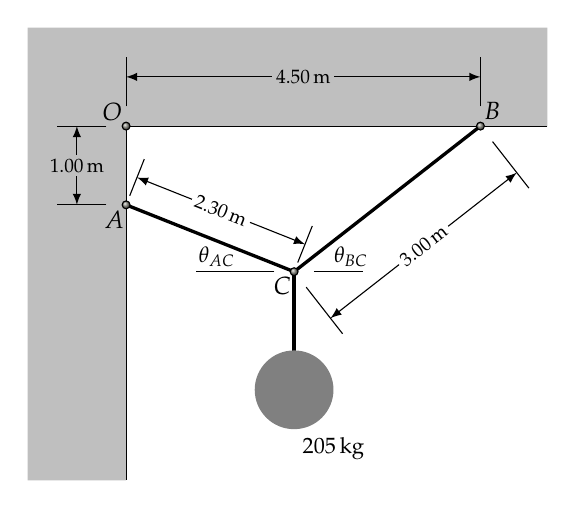
\begin{tikzpicture}[scale=1]

	\coordinate (O) at (0,0);
	\coordinate (B) at (4.5,0);
	\coordinate (BB) at ($(B)+(218:10)$);
	\coordinate (A) at (0,-1);
	\coordinate (AA) at ($(A)+(-21.7:10)$);
	% super cool tikzlibrary{calc} to get the intersection
	\coordinate (C) at (intersection of A--AA and B--BB);
	\coordinate (D) at ($ (C)+(0,-1.5) $);

	\fill[gray!50] (O) -- ($ (B)+(0.85,0) $) --+(0,1.25)--(-1.25,1.25) -- (-1.25, -4.5) -- +(1.25,0)--cycle;
	\draw[thin] ($ (B)+(0.85,0) $) -- (O) -- ($ (A)+(0,-3.5) $);
	\draw[very thick] (A)--(C);
	\draw[very thick] (B)--(C);
	\draw[very thick] (C)--(D);
	\fill[gray] (D) circle (.5cm);
	\node at ($ (C)-(-0.5,2.25) $) {\footnotesize $ 205\,$kg};

	\draw[thin] ($ (C)+(0.25,0) $) --+(0.625,0);
	\draw[thin] ($ (C)+(-0.25,0) $) --+(-1,0);
	\node at ($ (C)+(15:0.75) $) {\footnotesize $ \theta_{BC} $};
	\node at ($ (C)+(169:1) $) {\footnotesize $ \theta_{AC} $};

	\draw[thin]  ($ (O)+(-0.25,0) $) --+(-0.625,0);
	\draw[thin]  ($ (A)+(-0.25,0) $) --+(-0.625,0);
	\draw[latex-latex] ($ (O)+(-0.625,0) $) -- node[fill=gray!50, inner sep=0.5mm] {\scriptsize $1.00\,\text{m}$}($ (A)+(-0.625,0) $);

	
	\draw[thin]  ($ (O)+(0,0.25) $) --+(0, 0.625);
	\draw[thin]  ($ (B)+(0,0.25) $) --+(0, 0.625);
	\draw[latex-latex] ($ (O)+(0,.625) $) -- node[fill=gray!50, inner sep=0.5mm] {\scriptsize $4.50\,\text{m}$}($ (B)+(0,0.625) $);

	
	
	\draw[thin]  ($ (C)+(-52:0.25) $) --+(-52:.75);
	\draw[thin]  ($ (B)+(-52:0.25) $) --+(-52:.75);
	\draw[latex-latex] ($(C)+(-52:0.75)$) -- node[fill=white, sloped, inner sep=0.5mm] {\scriptsize $3.00\,\text{m}$}($(B)+(-52:0.75)$);
	\draw[thin]  ($ (A)+(68.3:0.125) $) --+(68.3:0.5);
	\draw[thin]  ($ (C)+(68.3:0.125) $) --+(68.3:0.5);
	\draw[latex-latex] ($(A)+(68.3:0.375)$) -- node[fill=white, sloped, inner sep=0.5mm] {\scriptsize $2.30\,\text{m}$}($(C)+(68.3:0.375)$);

  
	\small
	\fill [draw=black, ball color = Ivory4] (O) circle (0.05cm) node[black, xshift=-0.175cm, yshift=0.175cm] { $O$};
	\fill [draw=black, ball color = Ivory4] (B) circle (0.05cm) node[black, xshift=0.15cm, yshift=0.1875cm] {$B$};
	\fill [draw=black, ball color = Ivory4] (A) circle (0.05cm) node[black, xshift=-0.15cm, yshift=-0.1875cm] {$A$};
	\fill [draw=black, ball color = Ivory4] (C) circle (0.05cm) node[black, xshift=-0.15cm, yshift=-0.1875cm] {$C$};



\end{tikzpicture}
}
	}
\end{textblock*}

\begin{textblock*}{4.125in}(1in, 4.45in)
	\large
	\cbox{
		{\bf 22)} Find $\theta_{AC}$.\qquad\qquad
		{\bf 23) } Find $\theta_{BC}$.
		\begin{align*}
			AB^2 &= OA^2+OB^2 \\
			&= (1.00\,\mathsf{m})^2+(4.50\,\mathsf{m})^2 \\
			\Rightarrow AB &= 4.6098\,\mathsf{m}\\[0.5em]
			\cos \angle ACB &= \frac{AB^2+BC^2-AB^2}{2(AB)(BC)} \\
			&= \frac{(2.30\,\mathsf{m})^2+(3.00\,\mathsf{m})^2-(4.6098\,\mathsf{m})^2}{2(2.30\,\mathsf{mm})(3.00\,\mathsf{m}^2)} \\
			\Rightarrow \angle ACB &= 120.29\deg 
			% \angle OBA &= \tan^{-1}\left(\frac{1.00\,\mathsf{mm}}{4.50\,\mathsf{mm}}\right)=12.529\deg \\[0.5em]
			% \frac{\sin \angle ABC}{AC}  
		\end{align*}
	}
\end{textblock*}

\begin{textblock*}{6.75in}(1in, 7in)
	\large
	\cbox{
		\vspace{-0.75em}					
			$$\angle OBA = \tan^{-1}\left(\frac{1.00\,\mathsf{m}}{4.50\,\mathsf{m}}\right)=12.529\deg $$
			$$
			\frac{\sin  ABC}{AC} = \frac{\sin  ACB}{AB} \Rightarrow \frac{\sin  ABC}{2.30\,\mathsf{m}} = \frac{\sin  120.29\deg}{4.6098\,\mathsf{m}} \Rightarrow \angle ABC = 25.520\deg
			$$

			$$ \theta_{BC} = \angle OBA + \angle ABC = 12.259\deg+25.520\deg = 38.049\deg \qquad\text{(Alternate angles.)}$$

			$$ \theta_{AC} = 180\deg - \angle ACB - \theta_{BC} =180\deg-120.29\deg-38.049\deg = 21.661\deg $$

			$$\bm{\theta_{AC}=21.7\deg,\quad\theta_{BC}=38.0\deg }$$
	}
\end{textblock*}


%%%%%%%%%%%%%%%%%%%%%%%%%%%%%%%%%%%%%%%%%%%%%%%%%%%%%%%%%%%%%%%%%%%%%%%%%%%%%%%%%%%%%%%%%%%%%%%%%%%%
% page 7
%%%%%%%%%%%%%%%%%%%%%%%%%%%%%%%%%%%%%%%%%%%%%%%%%%%%%%%%%%%%%%%%%%%%%%%%%%%%%%%%%%%%%%%%%%%%%%%%%%%%
.\newpage



\begin{textblock*}{6.775in}(1in, 0.225in)
	\large
	\cbox{
		\mini[0.45]{
			\centering
      {\bf 24)} and {\bf 25)} Find the values of $\bm x$ and  $\bm y$ in the system shown.
    }
		\hfill
    \mini[0.5]{
      \vspace{-0.625cm}
      \begin{align}
        0.36911x + 0.61633y & = 2011.1 \\
        0.78748y - 0.92938x & = 0
      \end{align}
    }
    \parb
   From (2),
		\begin{equation}
			y = \frac{0.92938}{0.78748}x  = 1.1802x
		\end{equation}
    Substitute in (1) to find $x$
		\begin{align*}
			0.36911x + 0.61633(1.1802x) & = 2011.1 \\[0.5em]
			\Rightarrow \left(0.36911+0.61633(1.1802)\right)x & = 2011.1 \\[0.5em]
			\Rightarrow x & = \frac{2011.1}{\left(0.36911+0.61633(1.1802)\right)} \\
										& = 1834.1 \\
						\bm x		& \bm{=1830}
		\end{align*}
		
		Substitute back in (3) for $y$
		\begin{align*}
			0.78748y -0.92938(1834.1) & = 0         \\
			y                         & = 	2164.6   \\
			 \bm y                    & \bm{=2160}
		\end{align*}
  }  
\end{textblock*}


\begin{textblock*}{6.775in}(1in, 4.875in)
	\large
	\setcounter{equation}{0}
	\cbox{
    
    
    \mini[0.4]{
      {\bf 26)} and {\bf 27)} Determine $F_{AC}$ and  $F_{BC}$
    }
		\hfill
		\mini[0.5]{
      \vspace{-0.625cm}
      \begin{align}
        F_{BC}\sin15\deg + F_{AC}\cos35\deg + 1030.1 & = 0 \\
				F_{BC}\cos 15\deg+F_{AC}\sin35\deg           & = 0
      \end{align}
    }
		\parm
    From (2)
		\begin{align}
			F_{BC} & = -\frac{\sin 35^\circ}{\cos 15^\circ}F_{AC} = -0.59381F_{AC}
		\end{align}
		Substitute into (1)
		\begin{align*}
			\left(-0.59381F_{AC}\right)\sin{15^\circ}+F_{AC}\cos 35^\circ &= -1030.1\\[0.5em]
			-0.15369F_{AC}+0.81915F_{AC} &= -1030.1\\[1em]
			\Rightarrow F_{AC} &= \frac{-1030.1}{-0.15369+0.81915}\\
			&= -1548.0\\
			&= \bm{-1550}
		\end{align*}
		Substitute back into (3)
		\begin{equation*}
			F_{BC} = -0.59381(-1548.0) = 919.19 = \bm{919}
		\end{equation*}
  }  
\end{textblock*}



\end{document}